\section{Results}
We evaluated our models on data collected from the California Report Card between January 18th to April 20th.
We adminstered our reference survey through SurveyMonkey between March 8th and March 14th.
We consider a set of 1575 total participants from the CRC and a sample of 611 SurveyMonkey participants whose grading activity was as follows:

\begin{tabular}[!ht] { l | r | r | r | l }
Issue & No Change & Change & Skip & Median \\
\hline
\hline
  \multicolumn{5}{l}{\textbf{CRC}}\\
  \hline
  Obamacare & 749 & 223 & 593 & B \\
  \hline
  K12 & 849 & 172 & 544 & C+ \\
  \hline
  College & 923 & 139 & 503 & C-\\
  \hline
  Immigration & 693 & 105 & 767 & C \\
  \hline
  Marijuana & 881 & 118 & 566 & C \\
  \hline
  Marriage Rights & 929 & 105 & 531 & B+\\
\hline
\hline
\multicolumn{5}{l}{\textbf{Reference}}\\
\hline
  Obamacare & 498 & - & 113 & B \\
  \hline
  K12 & 561 & - & 50 & C \\
  \hline
  College & 573 & - & 38 & C-\\
  \hline
  Immigration & 375 & - & 236 & C+ \\
  \hline
  Marijuana & 498 & - & 113 & C \\
  \hline
  Marriage Rights & 554 & - & 57 & B+
\end{tabular}

For any given issue, between 10\% and 20\% of those who assigned grades registered a grade change.
In all, 556 out of the 1575 CRC participants changed their grades at least once (Figure \ref{change-1}).
\begin{figure}[h]
  \centering
    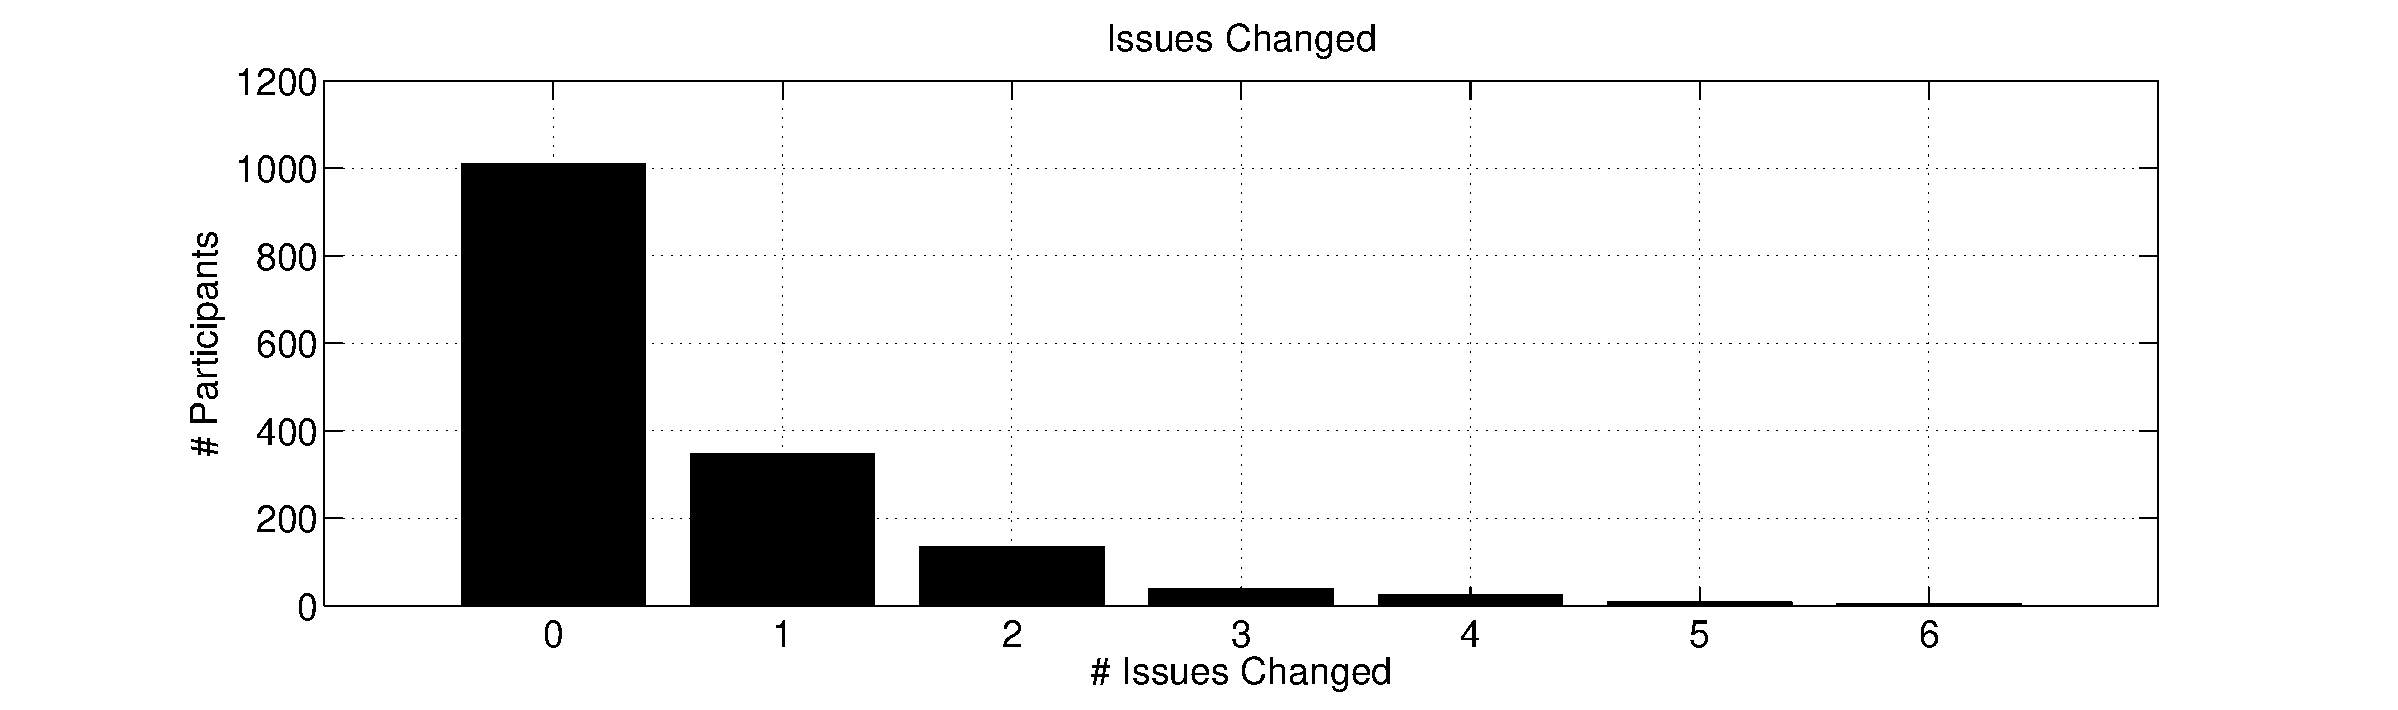
\includegraphics[scale=.40]{../plots/change-1.eps}
      \caption{The majority of participants did not change grades. 35\% of participants changed their grade on at least one issue, the majority of which (62\%) changed only a single issue. Less than 5\% of participants changed their grades on more than 4 out of the 6 issues.}
      \label{change-1}
\end{figure}
We also found that the aggregate results of the reference survey matched the CRC quite well.
On only two issues (K12 and Immigration), we found a observed differences which were both less than a letter grade (+ or -).

In our evaluation of these two surveys, we will use the unit \emph{full letter grades}.
For example, one full letter grade corresponds to the difference between an A grade and a B grade. 
A difference of a + or - is represented as $\frac{1}{3}$ eg. B to B+ or B+ to A-. 

\subsection{Social Herding Towards the Median}
Using the non-parametric test proposed in Section \ref{ht}, we tested the hypothesis of whether grade changes led to significantly more concentration around the median grade.
In our first experiment (Figure \ref{mdev-1}), we tested the absolute deviations of only the CRC users.
We compared the group of users that did not change their grades to the group that changed their grades.
We found that while there were no statistically significant differences between the initial grades of the two groups, the final grades of the group that changed were statistically significantly more concentrated than both their own initial grades and the grades of the no change group.
\begin{figure}[h]
  \centering
    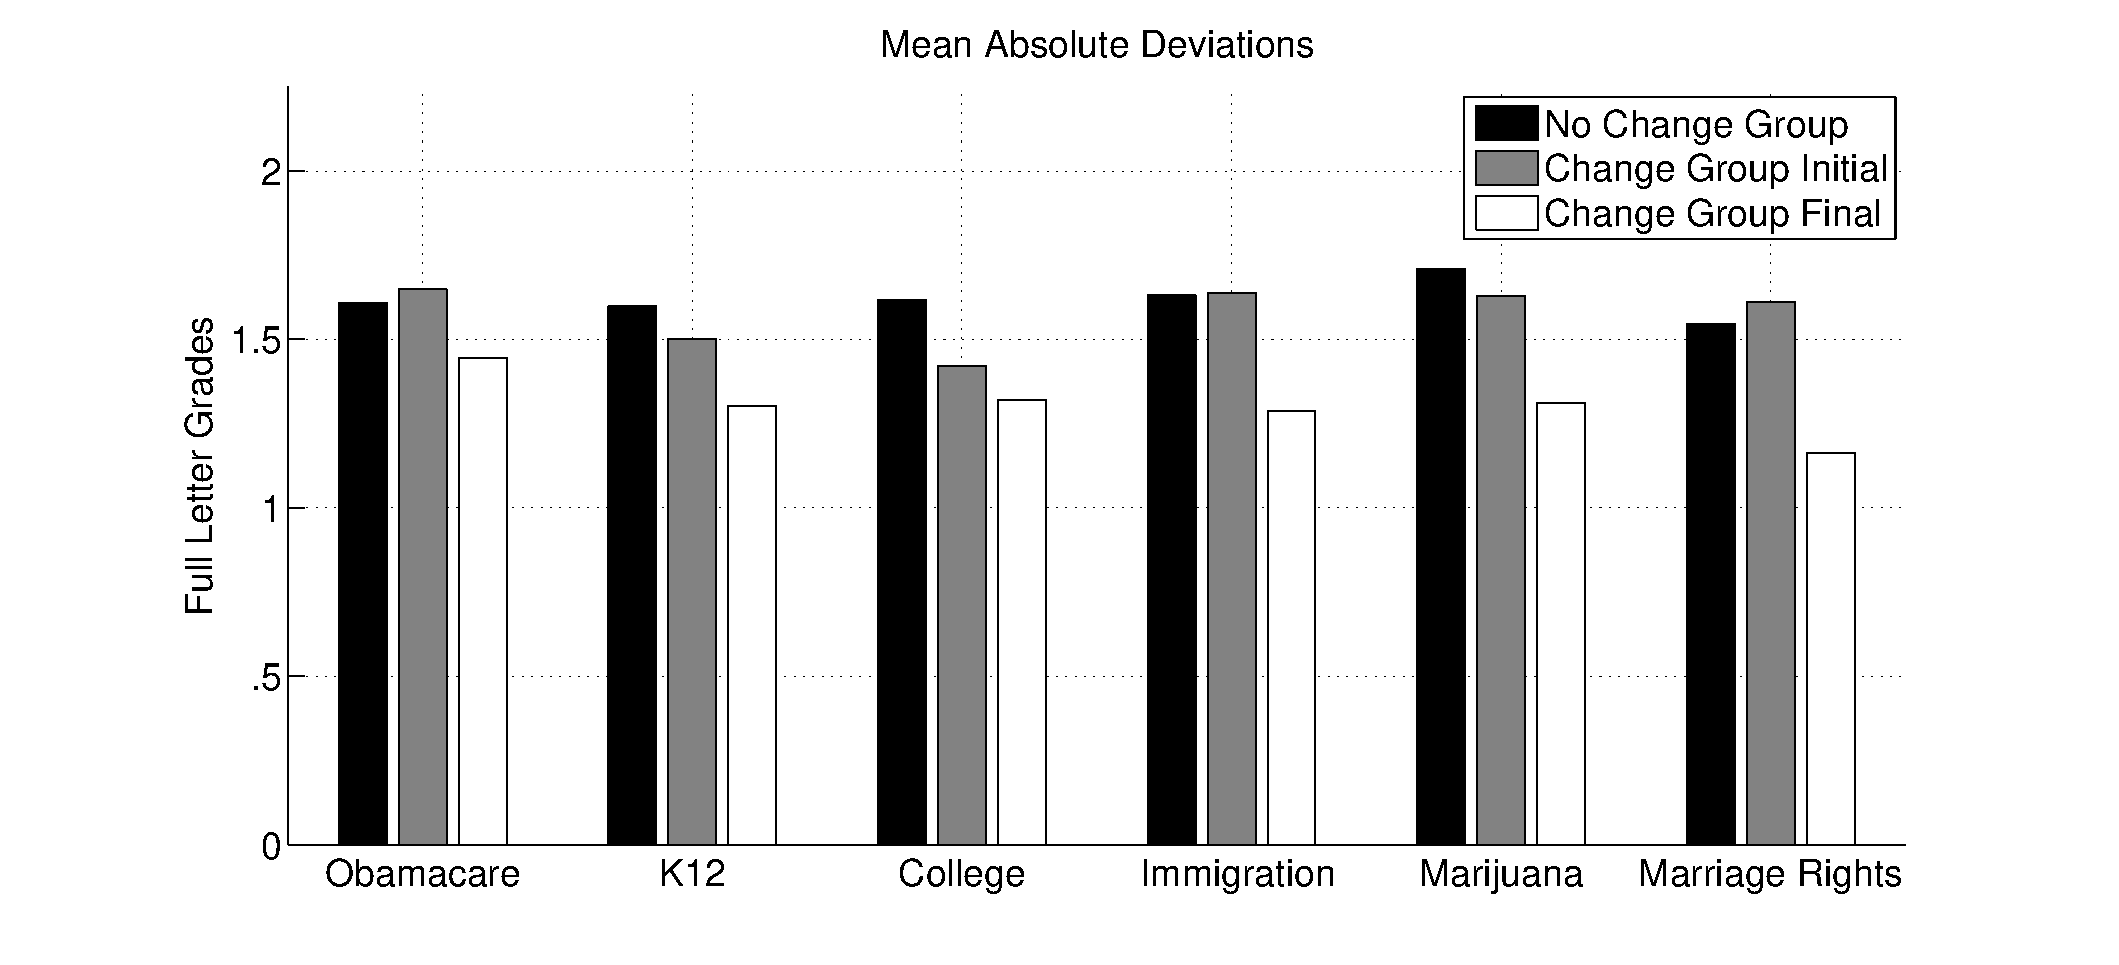
\includegraphics[scale=0.25]{../plots/abs-deviations-1.eps}
      \caption{For those users that changed their grades, final grades were significantly more concentrated around the median grade than their initial grades. In addition, these grades are more concentrated than the grades for those who didn't change.}
      \label{mdev-1}
\end{figure}

For the set of participants who changed their grades $P_c$ and those who did not $P_n$:

\begin{tabular}[!ht] { r | r | r }
\label{dev-2}
  Issue & p-val($P_c$ vs. $P_n$) & p-val($i$ vs. $f$) \\
  \hline
  \hline
  Obamacare &  0.0286 & 0.0161 \\
  \hline
  K12 & 2.1314e-06 &  0.0086 \\
  \hline
  College & 1.3033e-04 & 0.0415 \\
  \hline
  Immigration & 7.3456e-07 &4.4170e-05\\
  \hline
  Marijuana & 2.7549e-10 & 4.2560e-05\\
  \hline
  Marriage Rights & 3.5946e-06 & 2.4644e-10 \\
\end{tabular}

These results are consistent with the social herding hypothesis.
When participants change their grades, they are more likely to concentrate around the median.
What is particularly surprising is that the two groups of participants $P_n$ and $P_c$ are very similar in terms of intial grades, and the data suggests that herding is not correlated with more or less concentrated initial grades.

In our second experiment (Figure \ref{mdev-2}), we apply the same testing procedure to compare the grades from the CRC to to those in the reference survey.
We absolute deviations of the group of users who changed their grades in the CRC against users from the reference survey.
\begin{figure}[h]
  \centering
    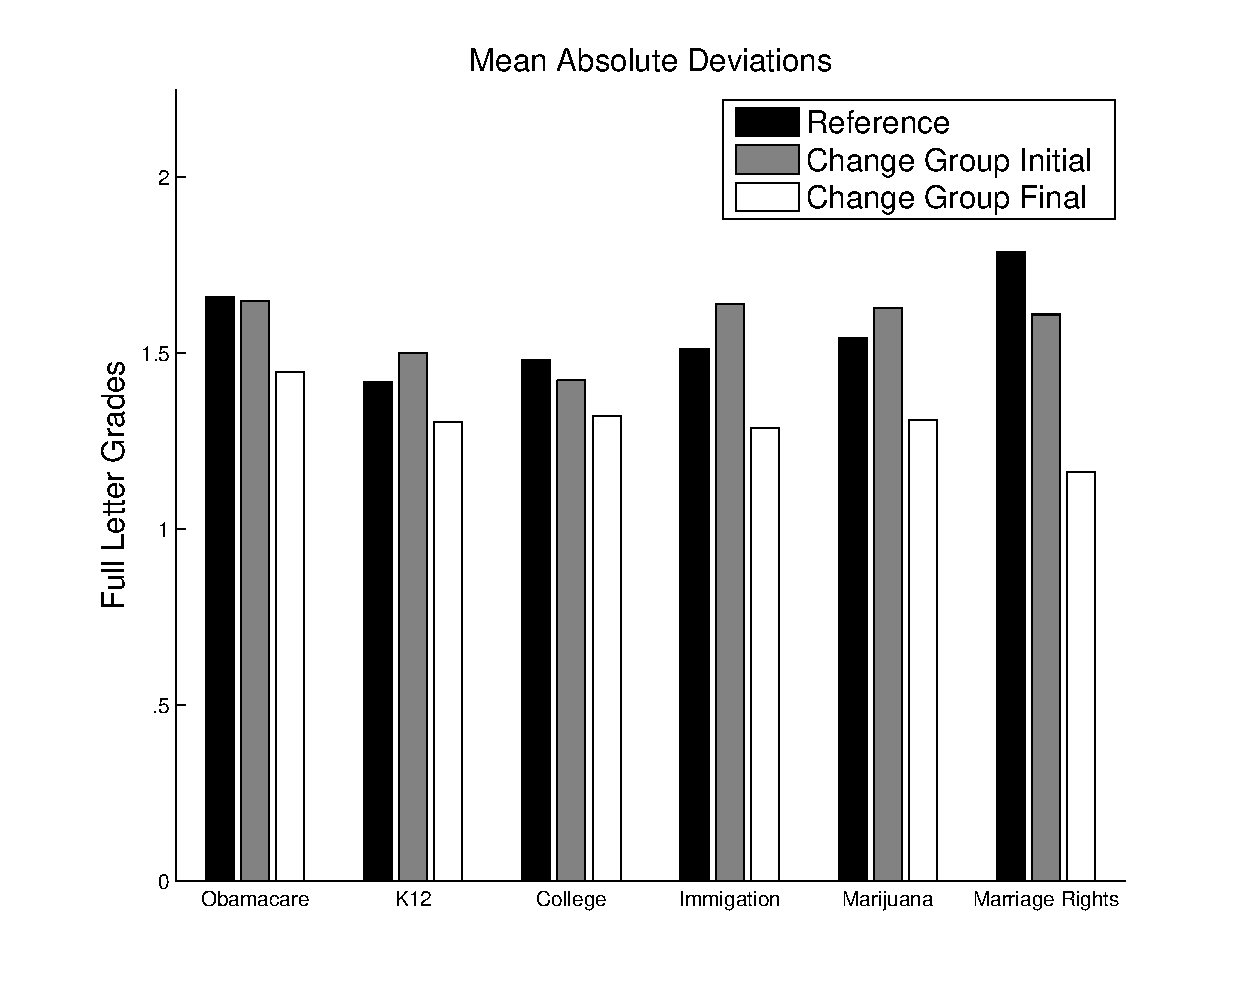
\includegraphics[scale=0.35]{../plots/bias-2.eps}
      \caption{We found that final grades were significantly more concentrated in the CRC compared to grades in the reference survey. Similar to Figure \ref{mdev-1}, we found that there was no statistically significant difference between the reference survey and the initial grades.}
      \label{mdev-2}
\end{figure}

\begin{tabular}[!ht] { r | r | r }
\label{ref-1}
  Issue & p-val($R$ vs. $i$) & p-val($R$ vs. $f$) \\
  \hline
  \hline
  Obamacare &  0.5386 & 0.0015 \\
  \hline
  K12 & 0.8283 & 0.0097 \\
  \hline
  College & 0.1452 & 0.0091 \\
  \hline
  Immigration & 0.3765 & 1.1787e-04\\
  \hline
  Marijuana & 0.7288 & 9.3111e-06\\
  \hline
  Marriage Rights & 0.2478 & 0.0161 \\
\end{tabular}

The results of our two experiments suggest that the CRC rating data is affected by social herding.
We not only found that participants' changed grades were statistically significantly more likely to concentrate around the median, they were also more likely in comparision to the reference survey.
While correlation does not imply causation, we argue that this evidence is most consistent with the social herding hypothesis.
As the CRC was not a randomized survey, there are possibly confounding covariates eg. participants who changed their grades were more likely to leave tightly concentrated grades in the first place.
However, our comparision with the reference survey, and discovery that initial grades were largely consistent with the reference survey and with those that didn't change their grades, suggest that these confounding covariates are not very significant.
These results are encouraging and we hope to run a randomized user study to confirm the causal relationship between revealing the median and concentrated grades.

\begin{figure}[ht!]
  \centering
    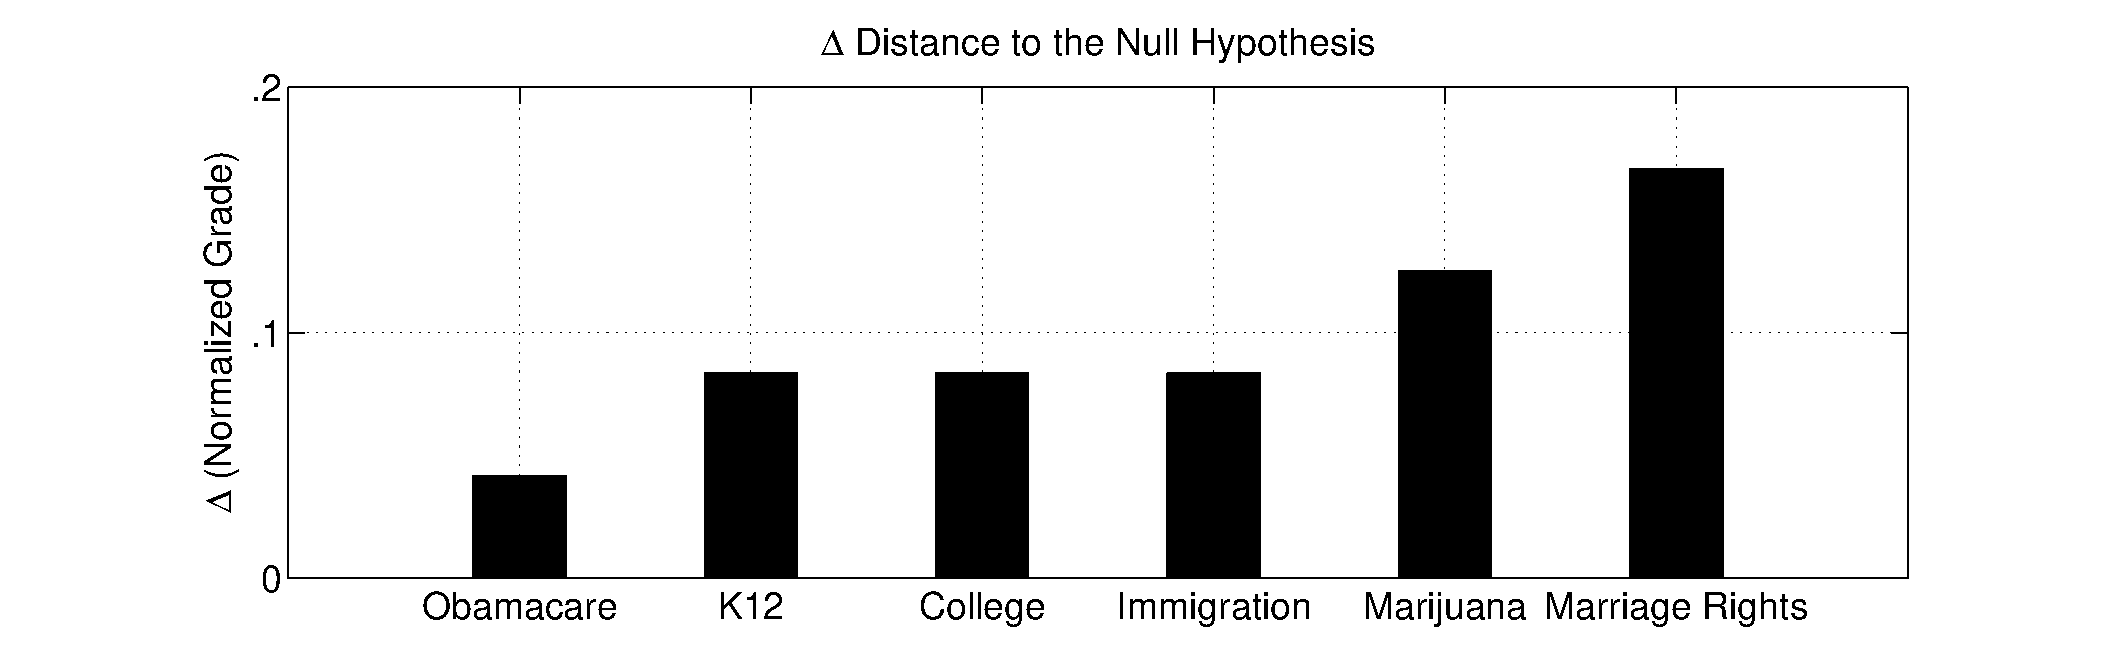
\includegraphics[scale=0.30]{../plots/shift-parameter.eps}
      \caption{We calculate the parameter $\Delta$ which is the most likely amount that our observations deviate from the null hypothesis. This can be interpreted as how much more are grades in our change group concentrated around the median.}
      \label{shift-1}
\end{figure}

\subsection{Social Herding Effects}
We tested the hypotheses and conclude significant additional concentration of grades around the median grade.
In Section \ref{ht}, we described how we could use the results of the hypothesis test to estimate the $\Delta$ parameter, which quantifies how different the hypothesis is from the null distribution.
In Figure \ref{shift-1}, we show the parameter estimates for each of the issues.
As before, the units of the plot are in terms of letter grades.
For the issues about Marriage Rights, we find that parameter is 2/3 of a letter grade.
This means that the set of absolute deviations for the change group $X_c$ was on average 2/3 of a letter grade smaller.
For the other issues, the parameter was smaller indicating less of an effect of social herding.
The parameter was the smallest for the first issue (Obamacare), and we conjecture that for this issue many participants were still learning how to use the slider interface; leading to random grade changes.
For this issue, we see that it had the most number of grade changes as well.

This parameter is very relevant to the design both recommender systems and predictive models.
Consider the problem of trying to predict a particpant's next grade.
The simplest model we could design is a model where we always select the median grade.
Such a model is often used as a baseline for comparision in recommender systems.
What we may interpret as low prediction error may in fact be the effects of social herding around the median, and if we were to apply this model asking the same questions but in a system without the herding effects; we may find that the same model performs poorly.
A median prediction is a naive model, but this problem affects many recommendation algorithms since they often rely on proximity metrics such as clustering, k-nearest neighbors, and some kernel machine learning methods.

\subsection{Sequence Dependence}
Using the model proposed in Section \ref{path}, we calculated the test statistics for both the CRC and the Reference Survey.
We found that for all issues the statistic was higher for the CRC suggesting an effect corroborating results in other work such as \cite{???}.
However, none of the results passed a $p < 0.05$ statistical significance test.
\begin{figure}[h!]
  \centering
    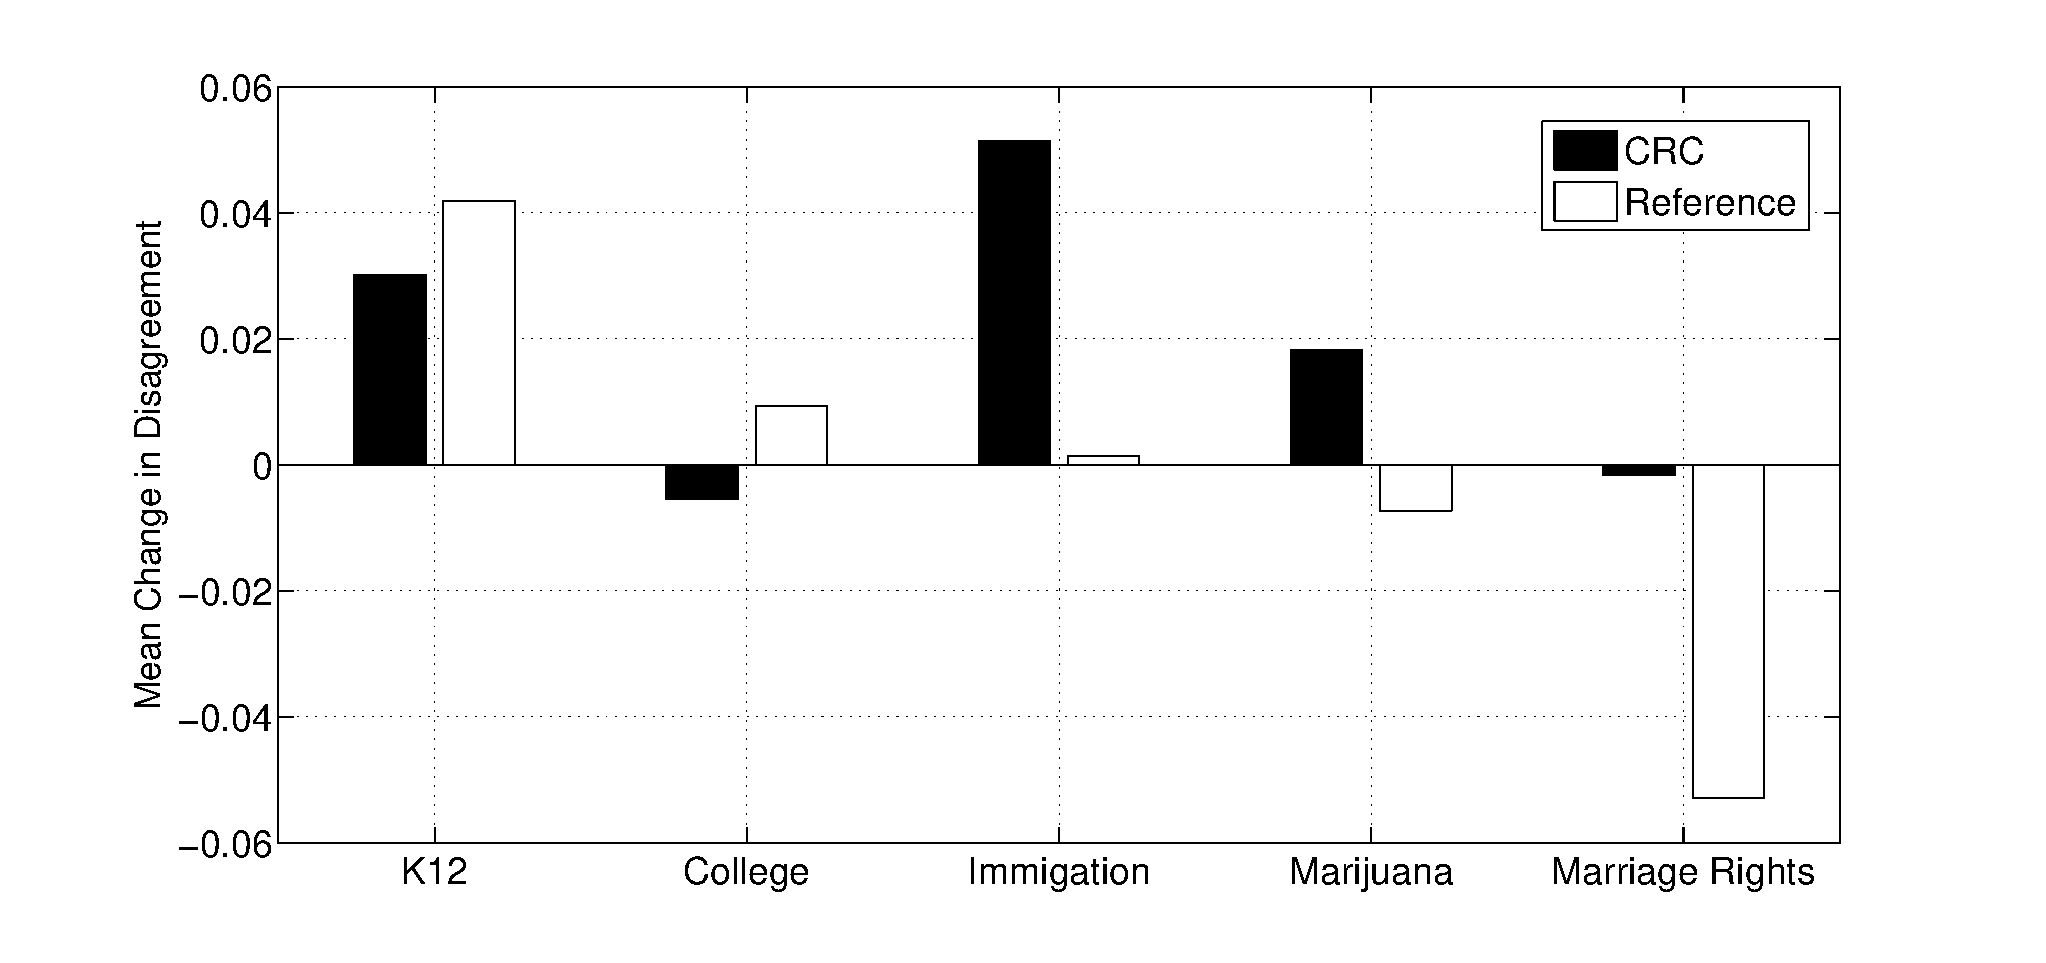
\includegraphics[width=\columnwidth]{../plots/path-dependence.eps}
      \caption{\textbf{TODO}}
      \label{path-1}
\end{figure}
We believe that these results suggest that there is some sequence dependence in the CRC, however, we cannot definitively conclude that from the current quantity of data.

\subsection{Grade Change Model}
In Figure \ref{opt-1} and Figure \ref{opt-2}, we show the results of our model search and locally optimal model for each issue.
We found for four out of the six issues, K12, College, Immigration, and Marijuana, the model we found was linear.
However, for Obamacare and Marriage Rights, we found that the relationship was quadratic.

\begin{figure*}[h!]
  \centering
    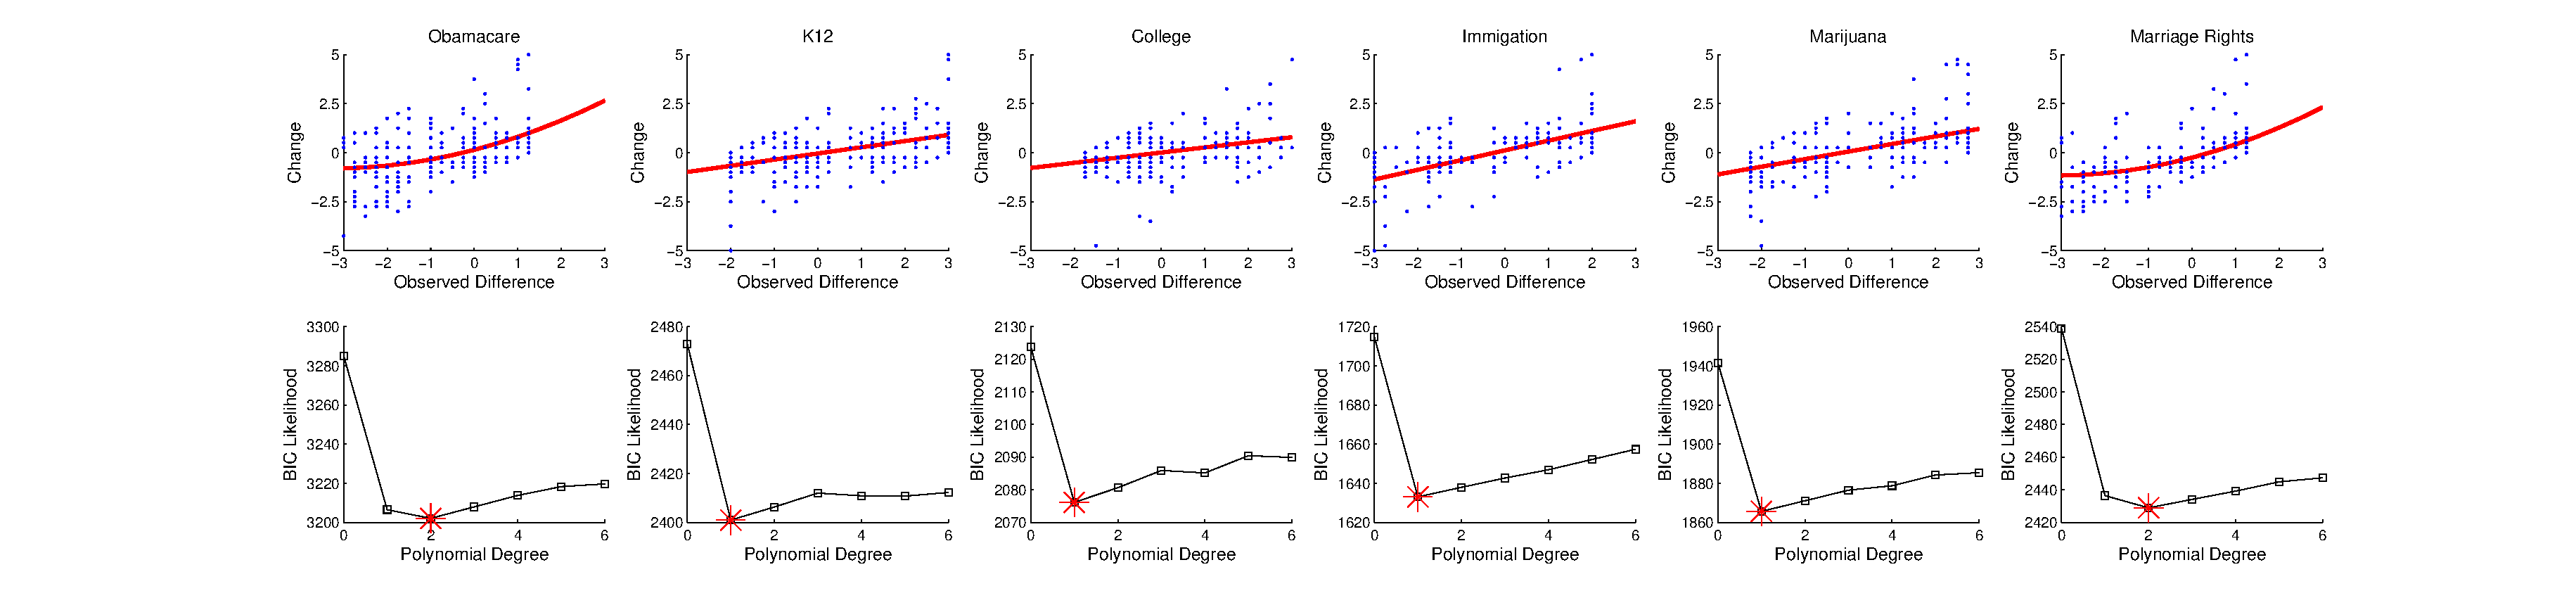
\includegraphics[scale=0.25]{../plots/BIC-optimization.eps}
      \caption{\textbf{TODO}}
      \label{opt-1}
\end{figure*}

\begin{figure*}[h!]
  \centering
    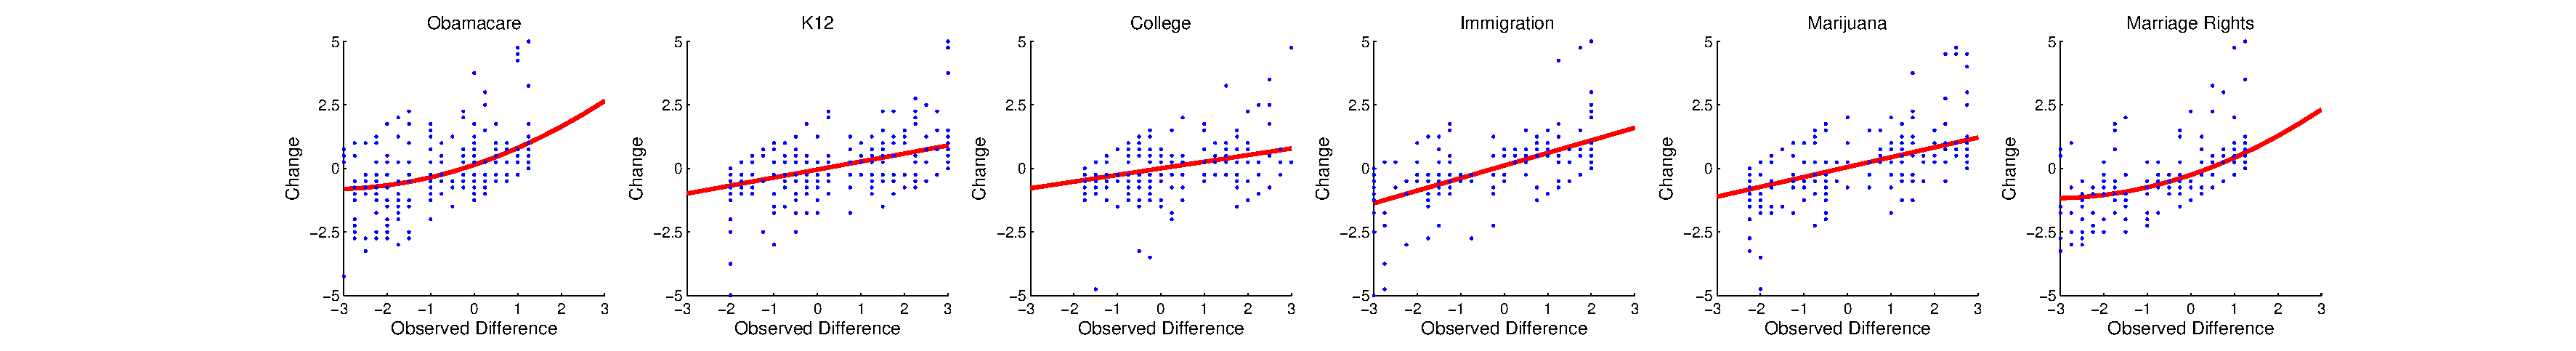
\includegraphics[scale=0.25]{../plots/BIC-optimization-2.eps}
      \caption{\textbf{TODO}}
      \label{opt-2}
\end{figure*}

Figure \ref{opt-2} illustrates the nature of the quadratic relationship, and we see heterogeneity between a positive regression towards the median and a negative regression.
Participants who initially graded the state higher than the median had a more significant tendency to regress downwards.
This result is interesting for a few reasons: (1) contrary to our initial expectations the relationship is largely linear and (2) non-linearities appear in the two issues that received the highest grades which also happen to be highly politicized issues.
There are many possible explanations for this including non-response bias \cite{???} or aversive response \cite{???}; and we defer a more detailed analysis to future work.

\subsection{Comparision To Reference Survey}
We applied our proposed non-parametric test to compare the absolute deviations in the group of participants who changed their grades in the CRC with results from a reference survey.
For the reference survey, we calculated the absolute deviation around the median (which the participants were not shown).
We found for all but one issue the grades from the CRC were statistically significantly closer to the median than ones from the reference survey.

\begin{tabular}[!ht] { r | l | l | r}
\label{ref-1}
  Issue & Med(Ref) & Med(CRC) & p-val \\
  \hline
  \hline
  Obamacare &  B & B & 0.0078\\
  \hline
  K12 & C+ & C & 0.3563\\
  \hline
  College & C- & C- & 0.0011\\
  \hline
  Immigration & C & C+ & 0.0277\\
  \hline
  Marijuana & C & C & 0.0076\\
  \hline
  Marriage Rights & B+ & B+ & 0.0494 \\
\end{tabular}

Furthermore, the two surveys aligned nearly perfectly in aggregate.
